% Scaffld: the 5-minute pitch deck (16:9). Build: latexmk -pdf deck.tex
\documentclass{article}
\usepackage[paperwidth=320mm, paperheight=180mm, margin=0mm]{geometry}
\usepackage[T1]{fontenc}
\usepackage[scaled=0.95]{helvet}
\renewcommand{\familydefault}{\sfdefault}
\usepackage{graphicx}
\graphicspath{{img/}{../media/}}
\usepackage{xcolor}
\usepackage{tikz}
\usetikzlibrary{calc, positioning}
\usepackage[hidelinks]{hyperref}
\hypersetup{pdftitle={Scaffld: pitch deck}, pdfauthor={Team Scaffld}}

\definecolor{bg}{HTML}{0D1016}
\definecolor{panel}{HTML}{1D212A}
\definecolor{ink}{HTML}{F2F2EE}
\definecolor{muted}{HTML}{9497A0}
\definecolor{blue}{HTML}{4A8FE6}
\definecolor{orange}{HTML}{EB6834}
\definecolor{green}{HTML}{26B474}
\pagecolor{bg}
\color{ink}
\pagestyle{empty}
\setlength{\parindent}{0pt}

\newcommand{\at}[2]{($(current page.north west)+({(#1)*1mm},{-(#2)*1mm})$)}
\newcommand{\T}[1]{\fontsize{#1pt}{\fpeval{1.22*#1}pt}\selectfont}
\newcommand{\slidetitle}[2][]{%
  \node[anchor=north west, inner sep=0, text width=290mm, align=left, font=\T{12}\bfseries, text=blue] at \at{16}{13} {#1};
  \node[anchor=north west, inner sep=0, text width=292mm, align=left, font=\T{30}\bfseries] at \at{16}{21} {#2};}
\newcommand{\foot}[1]{\node[anchor=south west, inner sep=0] at ($(current page.south west)+(16mm,8mm)$) {\T{10}\color{muted}#1\par};
  \node[anchor=south east, inner sep=0] at ($(current page.south east)+(-16mm,8mm)$) {\T{10}\color{muted}Scaffld \,·\, AgentVerse 2026\par};}
\newenvironment{slide}{\noindent\begin{tikzpicture}[remember picture, overlay]}{\end{tikzpicture}\newpage}
\newcommand{\card}[5]{% x, y, w, h, content
  \node[anchor=north west, fill=panel, rounded corners=3mm, minimum width=#3mm, minimum height=#4mm, inner sep=0] at \at{#1}{#2} {};
  \node[anchor=north west, text width=#3mm-12mm, align=left, inner sep=0] at \at{#1+6}{#2+6} {#5};}
\newcommand{\stat}[3]{{\T{#1}\bfseries\color{#2}#3\par}}

\begin{document}

% 1 ---------------------------------------------------------------------------------------------------------------
\begin{slide}
\node[anchor=north west, inner sep=0] at \at{16}{30} {\T{14}\bfseries\color{blue}AgentVerse 2026 \,·\, Robotics Track\par};
\node[anchor=north west, inner sep=0] at \at{16}{42} {\T{60}\bfseries Scaffld\par};
\node[anchor=north west, inner sep=0, text width=140mm, align=left, font=\T{24}] at \at{16}{68} {A robot teacher that finds the gaps in a robot's skills and builds its own lessons.};
\node[anchor=north west, inner sep=0, text width=140mm, align=left, font=\T{26}\bfseries, text=blue] at \at{16}{106} {One typed sentence $\rightarrow$\\a new robot skill in 39.7 minutes.};
\node[anchor=north west, inner sep=0, text width=140mm, align=left, font=\T{16}, text=muted] at \at{16}{138} {No human demonstrations. The trained student then runs alone on a laptop: no teacher, no cloud.};
\node[anchor=north east, inner sep=0] at \at{306}{26} {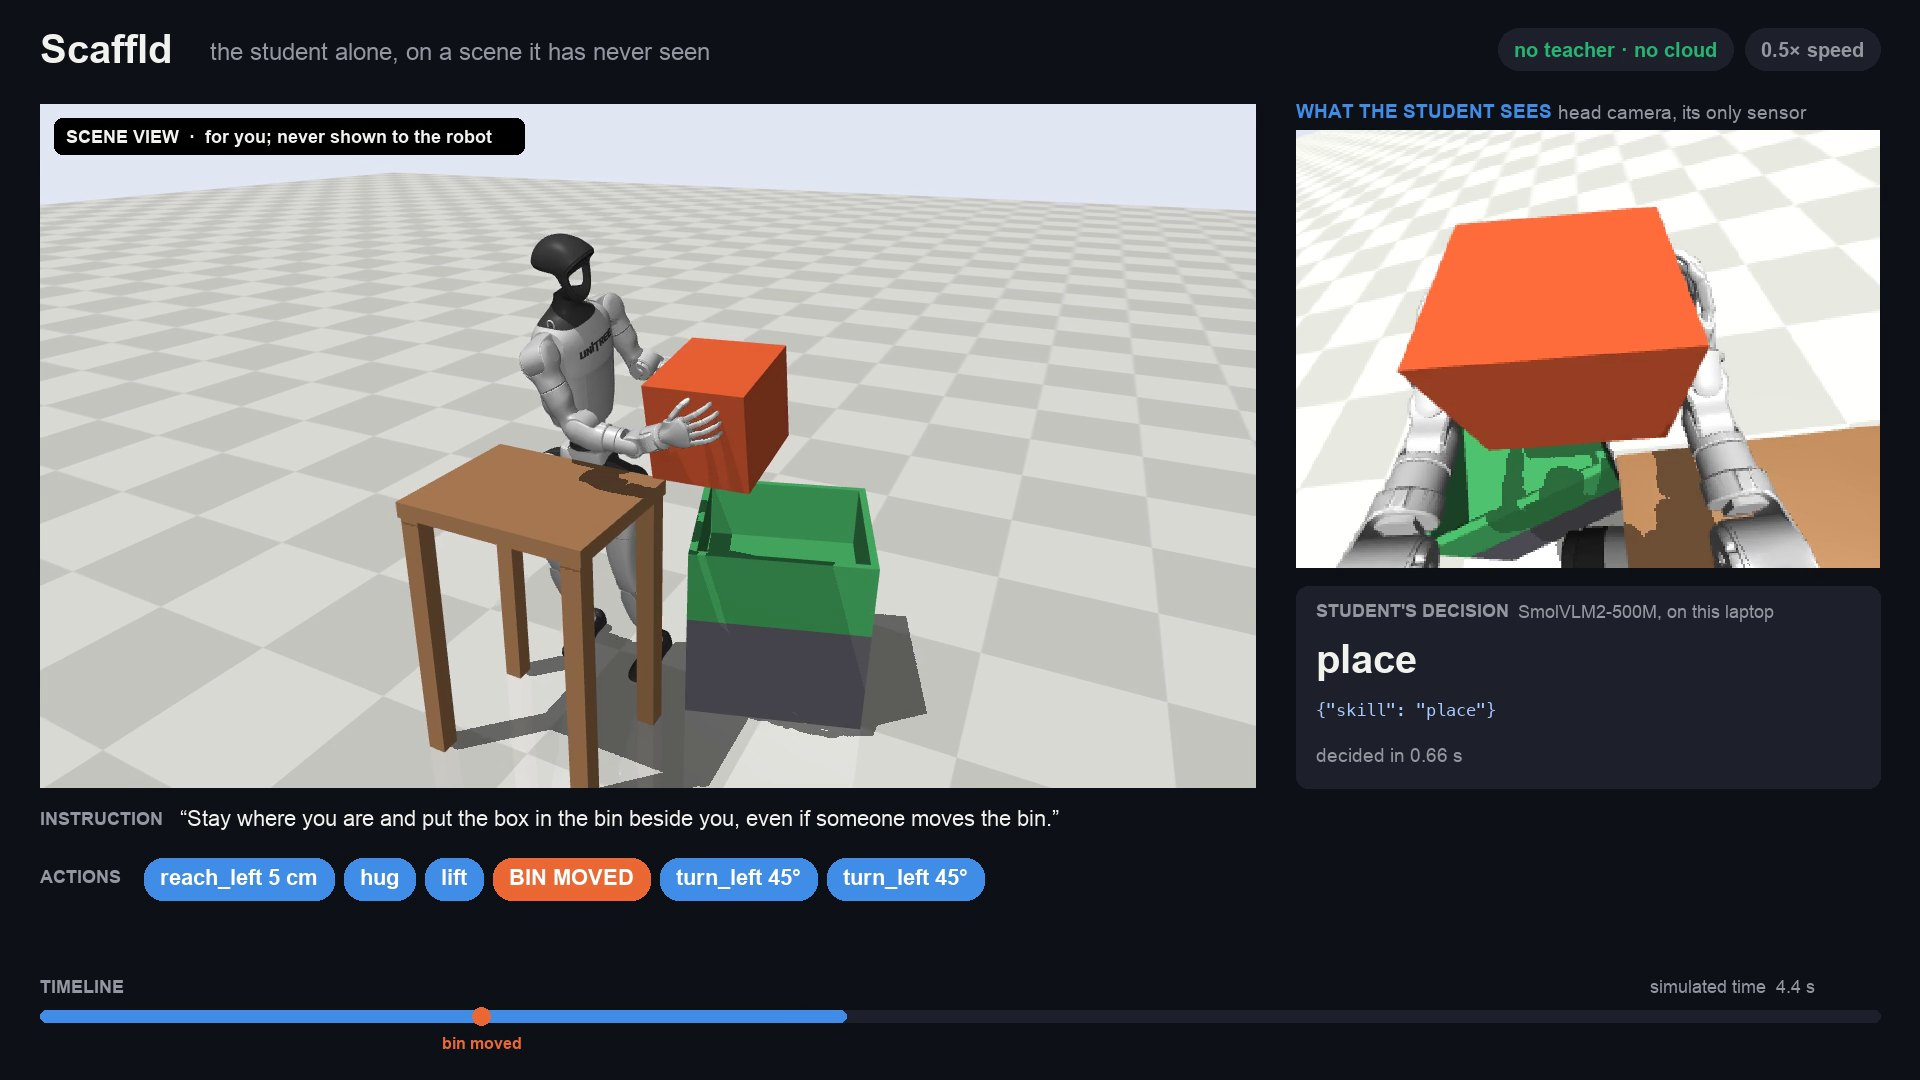
\includegraphics[width=146mm]{hero.jpg}};
\foot{Owen Yan \,·\, Isaac \,·\, Santi \,·\, Anh \,·\, Josh Lim \qquad github.com/owenbonc/isaac-s-mom}
\end{slide}

% 2 ---------------------------------------------------------------------------------------------------------------
\begin{slide}
\slidetitle[The problem]{Robots learn from human demonstrations.\\That doesn't scale.}
\card{16}{66}{138}{70}{\stat{40}{orange}{50 collectors}\par\vspace{1mm}\stat{40}{orange}{$\times$ 12 months}\par\vspace{4mm}{\T{18}to record 76k trajectories (DROID)\par}}
\card{166}{66}{138}{70}{\stat{40}{orange}{13 robots}\par\vspace{1mm}\stat{40}{orange}{$\times$ 17 months}\par\vspace{4mm}{\T{18}to collect 130k episodes (RT-1)\par}}
\node[anchor=north west, inner sep=0, text width=290mm] at \at{16}{146} {\T{20}Every new task, and every new failure, costs \textbf{more operator hours}.};
\foot{DROID: Khazatsky et al., arXiv:2403.12945. RT-1: Brohan et al., RSS 2023.}
\end{slide}

% 3 ---------------------------------------------------------------------------------------------------------------
\begin{slide}
\slidetitle[Our idea]{Let a teacher agent create the lessons.}
\card{16}{48}{91}{100}{\stat{14}{orange}{TEACHER \,·\, Argon, cloud}\par\vspace{4mm}\T{17}\textbf{Writes the task} from one sentence.\par\vspace{3mm}\textbf{Demonstrates} by driving the robot through its own camera and skills.\par\vspace{3mm}\textbf{Diagnoses} the student's failures and teaches the fix.}
\card{115}{48}{91}{100}{\stat{14}{green}{VALIDATOR \,·\, ground truth}\par\vspace{4mm}\T{17}\textbf{Judges every demo} by a declarative success rule.\par\vspace{3mm}\textbf{Keeps only what works}: unsafe or failed demos never train.\par\vspace{3mm}Says \textbf{why} a failure happened, in words.}
\card{214}{48}{90}{100}{\stat{14}{blue}{STUDENT \,·\, 500M, laptop}\par\vspace{4mm}\T{17}\textbf{Learns} from the accepted teacher steps (LoRA).\par\vspace{3mm}Sees \textbf{only the head camera}.\par\vspace{3mm}\textbf{Runs alone}: no teacher, no cloud, 0.31\,s per decision.}
\foot{Unitree G1 humanoid (29 DoF) in MuJoCo \,·\, 10 whitelisted skills behind a safety gate}
\end{slide}

% 4 ---------------------------------------------------------------------------------------------------------------
\begin{slide}
\slidetitle[How it works]{One sentence $\rightarrow$ a tested skill in \color{blue}39.7 minutes}
\node[anchor=north, inner sep=0] at \at{160}{44} {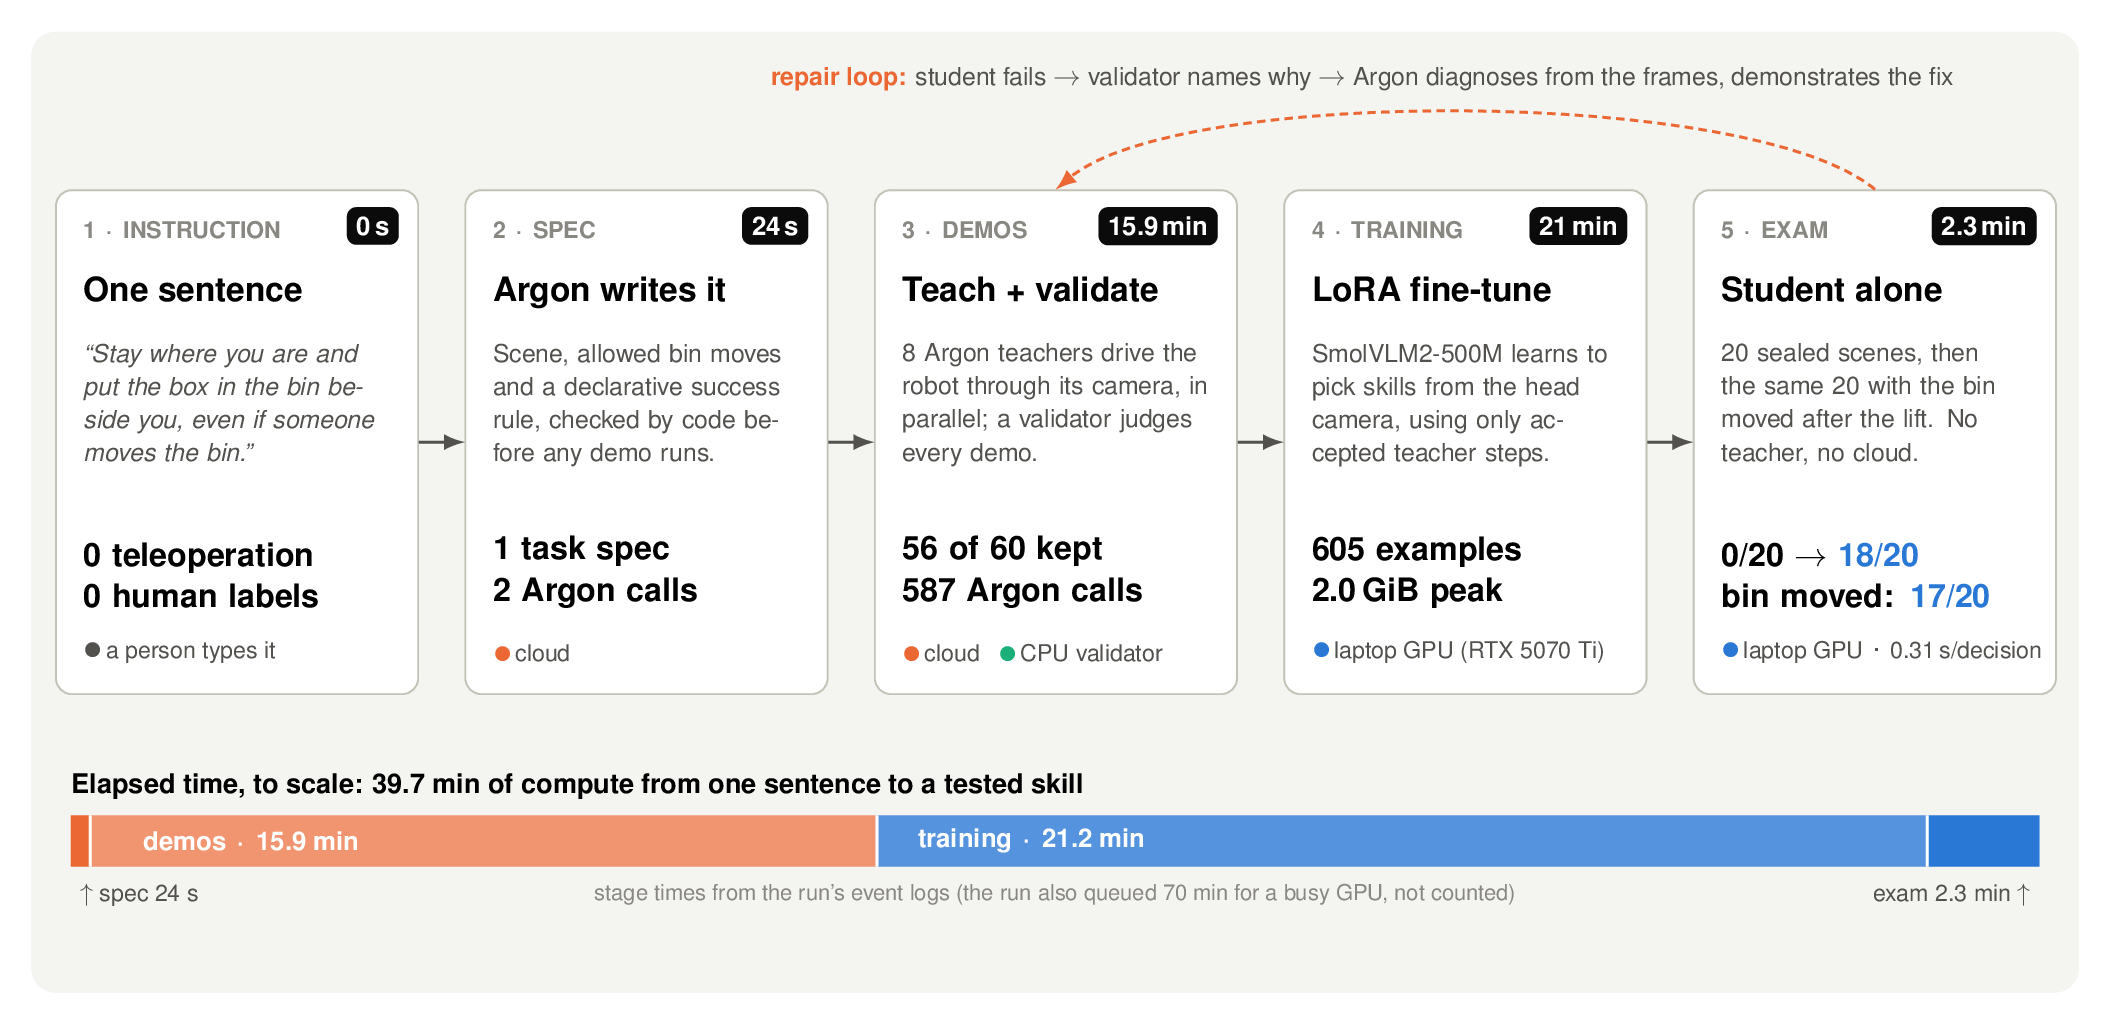
\includegraphics[width=250mm]{pipeline.png}};
\foot{Stage times measured from the run's event logs; a 70-minute wait for a busy GPU is not counted.}
\end{slide}

% 5 ---------------------------------------------------------------------------------------------------------------
\begin{slide}
\slidetitle[Watch]{The student alone. The bin moves mid-task.}
\node[anchor=north, inner sep=0] at \at{160}{42} {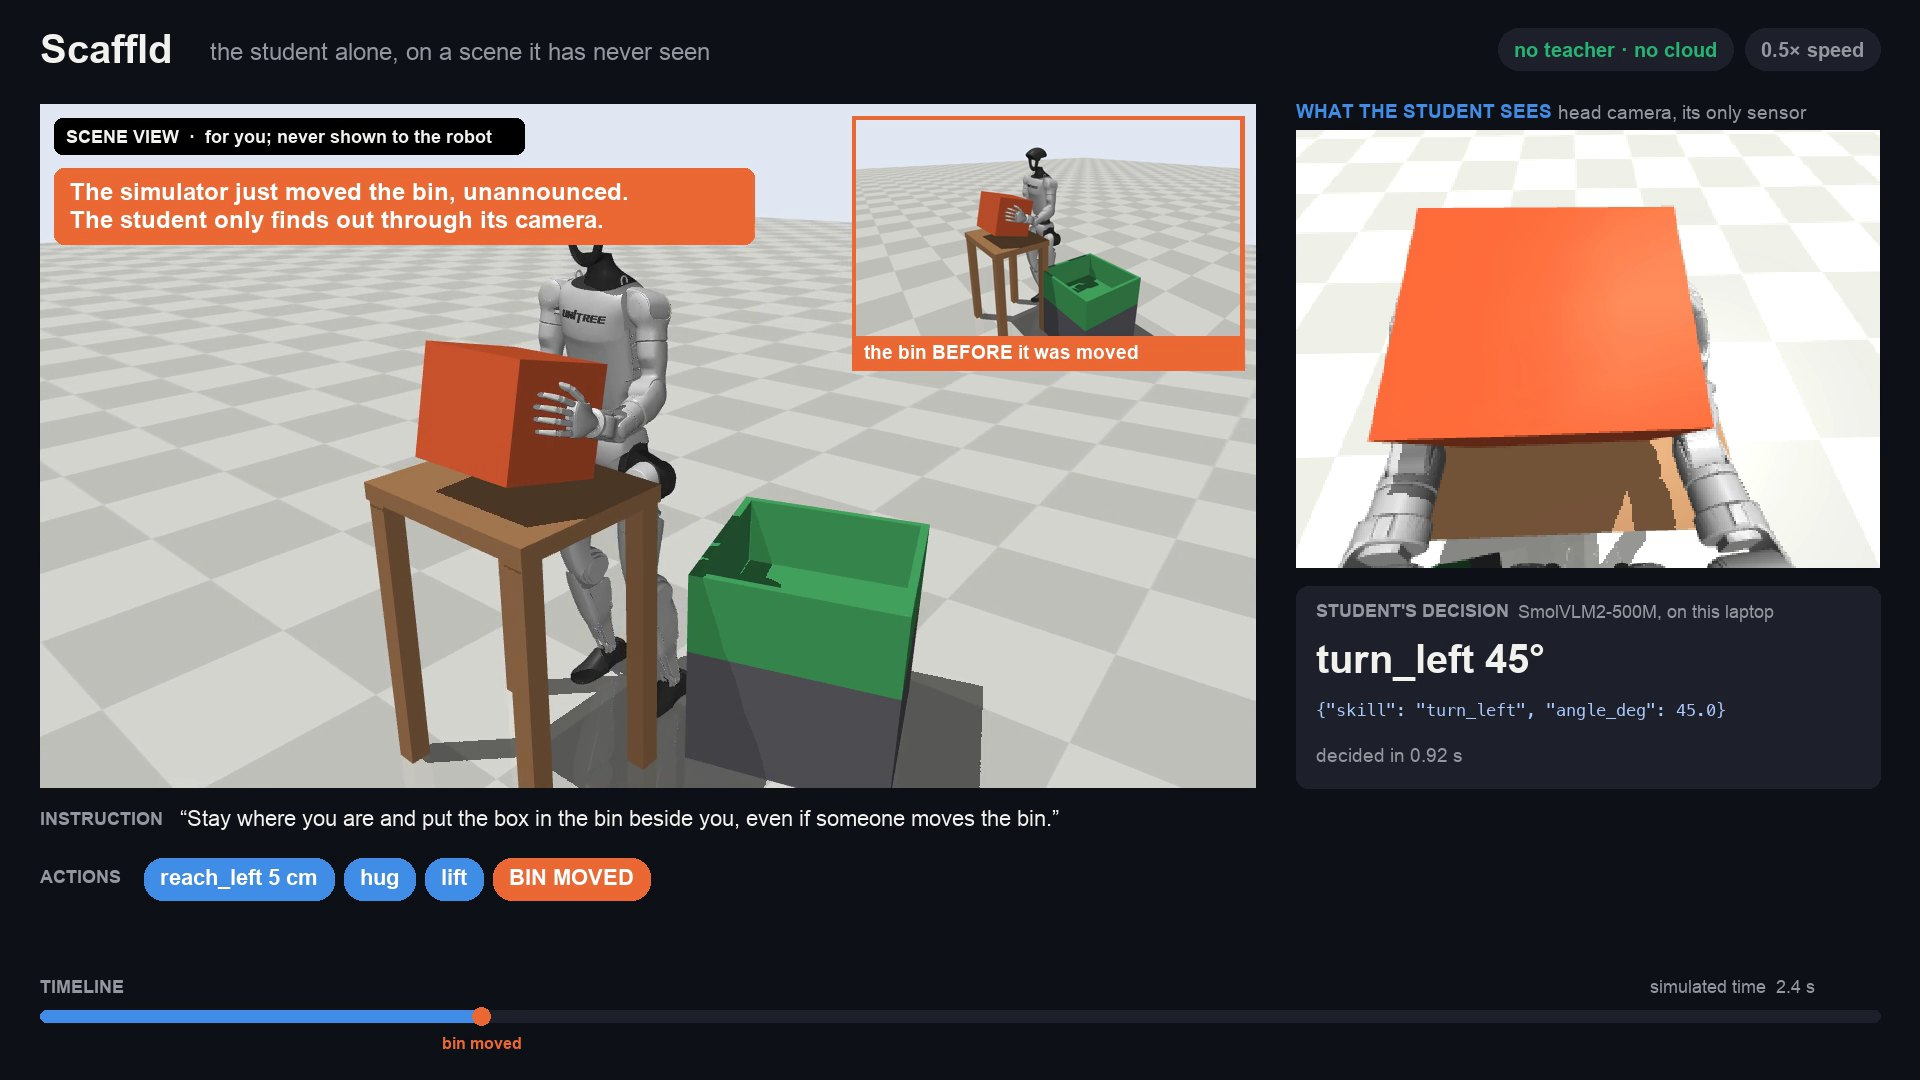
\includegraphics[width=204mm]{hero-move.jpg}};
\node[anchor=north, inner sep=0, text width=290mm, align=center] at \at{160}{161} {\T{15}\color{muted}One continuous take from the simulator \,·\, perception beside action \,·\, the simulator moves the bin, unannounced\par};
\end{slide}

% 6 ---------------------------------------------------------------------------------------------------------------
\begin{slide}
\slidetitle[Result 1]{From 0/20 to \color{blue}18/20\color{ink} on scenes it has never seen}
\card{16}{50}{120}{100}{\stat{56}{blue}{18/20}\par\vspace{1mm}{\T{17}sealed, unseen scenes, student alone\par}\par\vspace{6mm}\stat{40}{blue}{17/20}\par\vspace{1mm}{\T{17}with the bin moved after the lift\par}\par\vspace{6mm}{\T{17}\color{muted}untrained model: 0/20 and 0/20\par McNemar $p<0.001$, paired by seed\par\par}}
\node[anchor=north west, inner sep=0] at \at{146}{50} {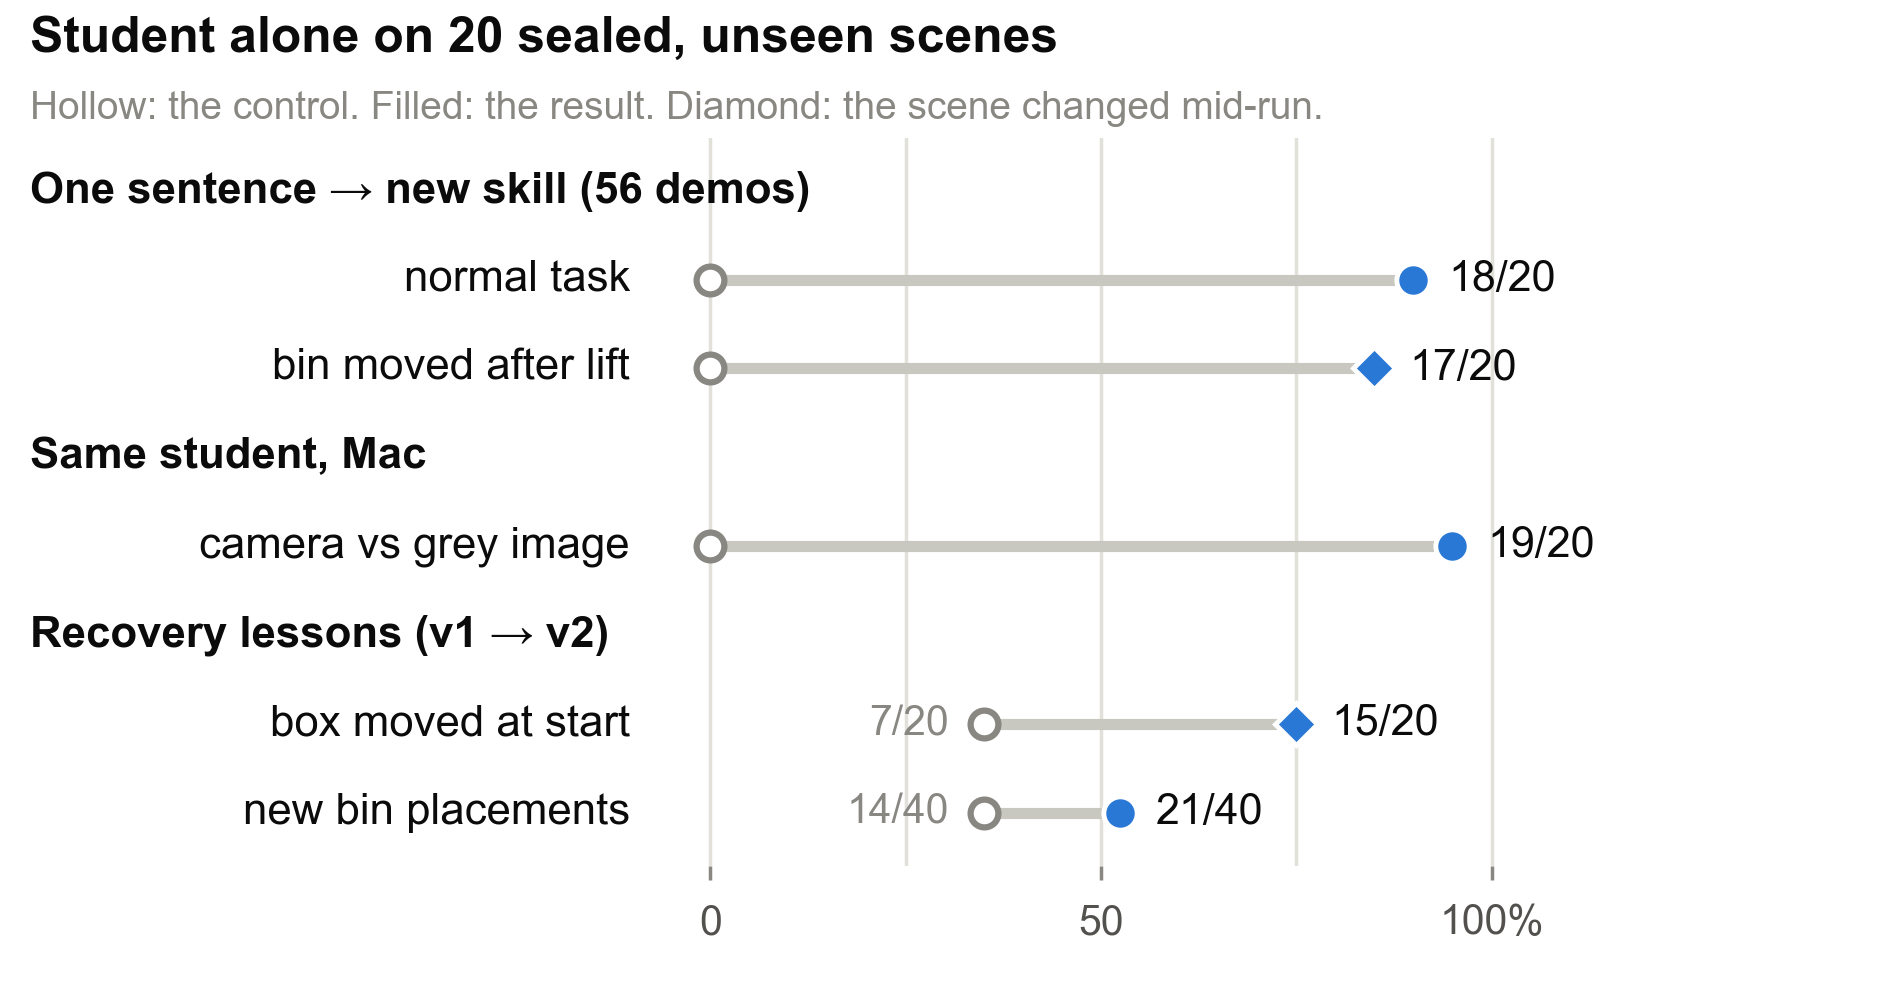
\includegraphics[width=158mm]{results-student.png}};
\foot{Trained on 56 accepted teacher demos (605 examples, 21-minute fine-tune). Every count traces to a saved episode.}
\end{slide}

% 7 ---------------------------------------------------------------------------------------------------------------
\begin{slide}
\slidetitle[Result 2]{It acts on what it sees.}
\node[anchor=north west, inner sep=0] at \at{16}{46} {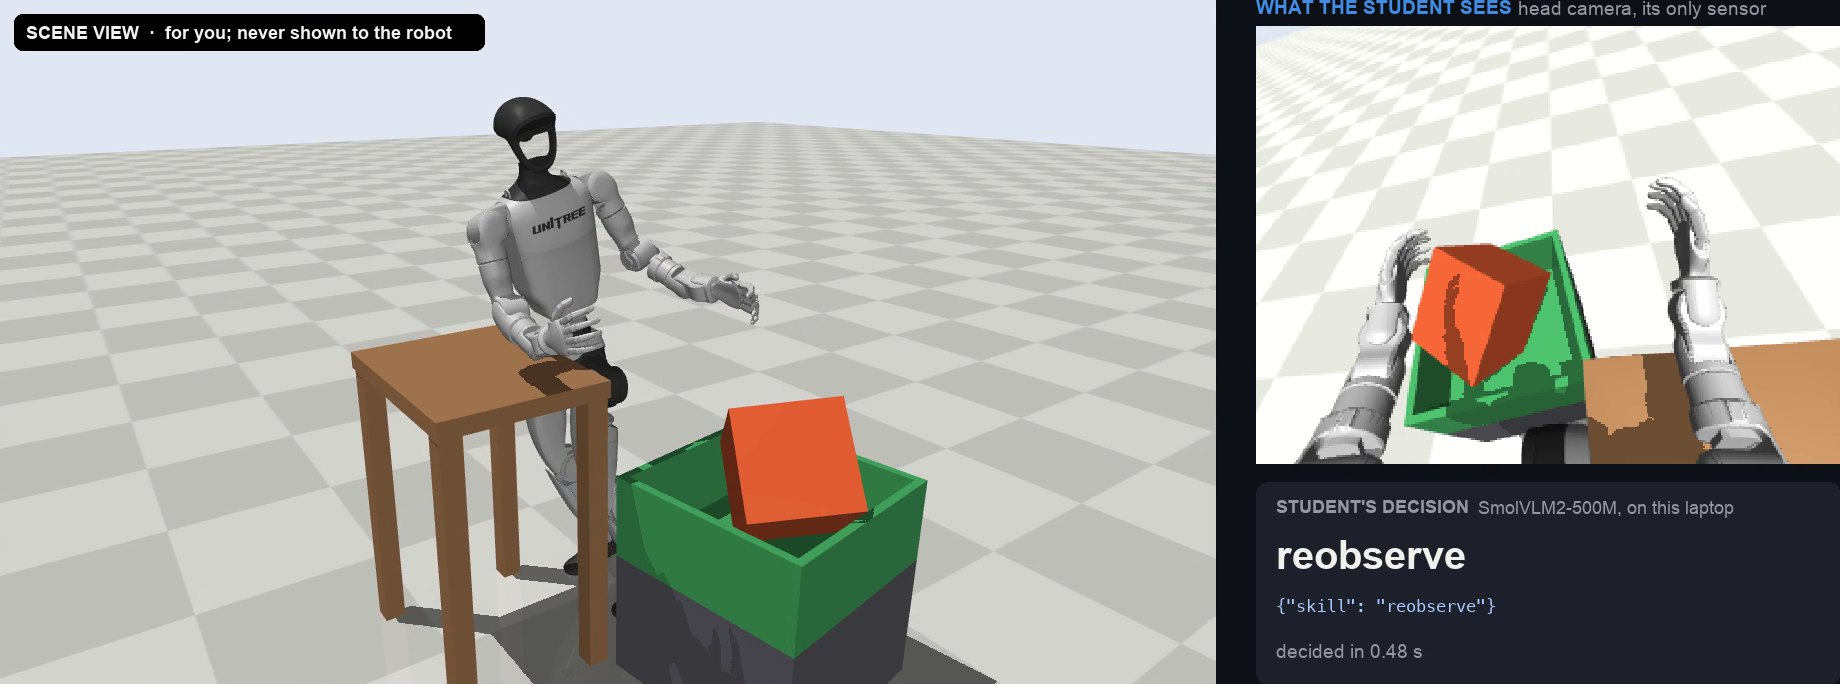
\includegraphics[width=142mm]{pair-camera.jpg}};
\node[anchor=north west, inner sep=0] at \at{162}{46} {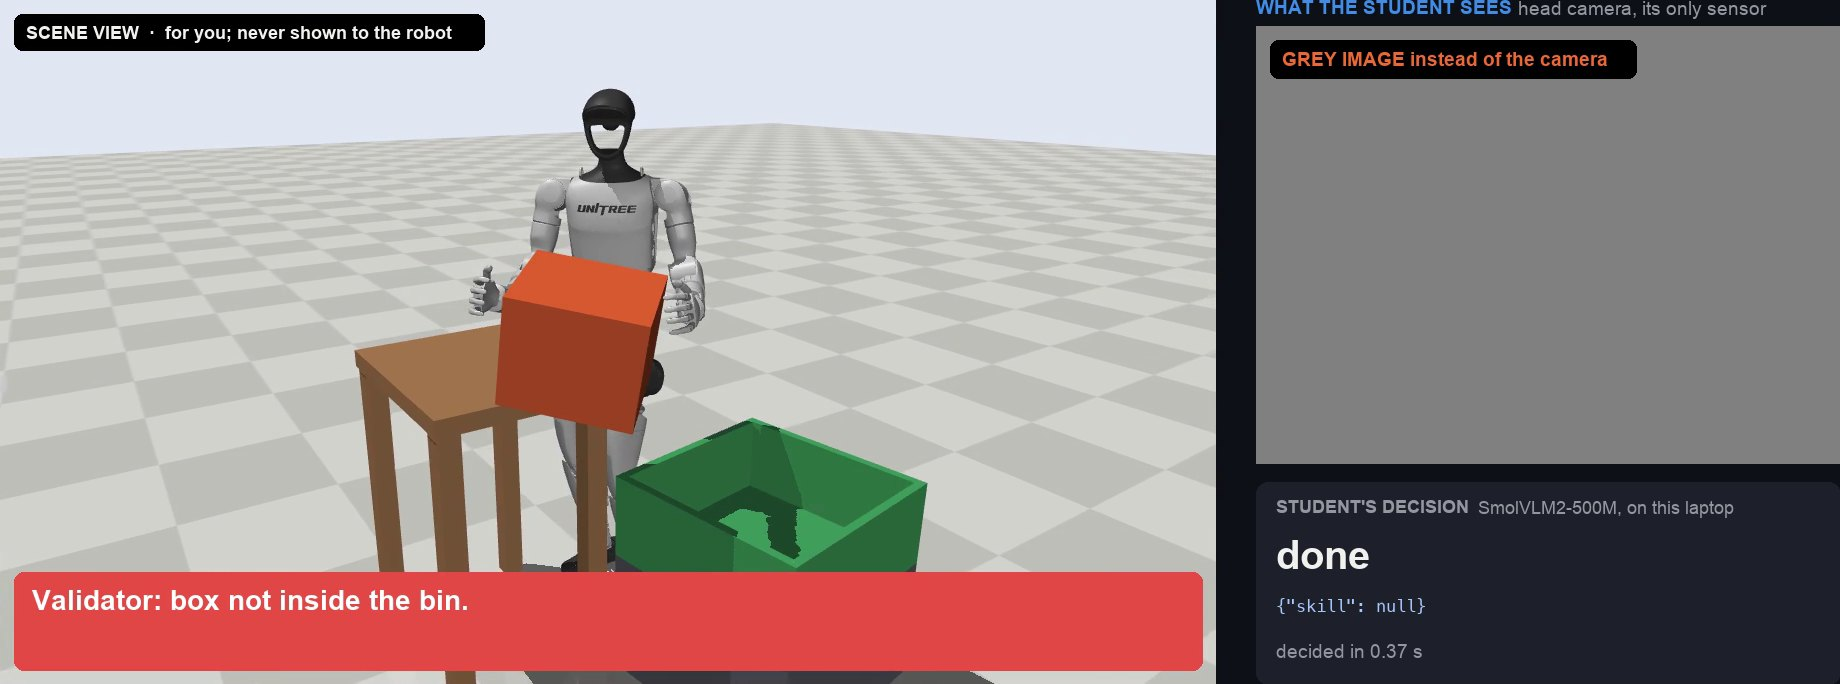
\includegraphics[width=142mm]{pair-grey.jpg}};
\node[anchor=north west, inner sep=0, text width=142mm] at \at{16}{102} {\stat{30}{green}{camera: 19/20}\par\vspace{1mm}{\T{16}It twists until the bin is under the box, then places.\par}};
\node[anchor=north west, inner sep=0, text width=142mm] at \at{162}{102} {\stat{30}{orange}{grey image: 0/20 (Mac)}\par\vspace{1mm}{\T{16}Same scene, same student: one twist, and it misses.\par}};
\node[anchor=north west, inner sep=0, text width=290mm] at \at{16}{134} {\T{18}\textbf{The demonstrations teach when to stop:} trained on 14 or 28 demos it never places (0/20); on 56, \textbf{18/20}.};
\foot{Camera vs grey image: same checkpoint, seeds and machine (Mac); only the image differs.}
\end{slide}

% 8 ---------------------------------------------------------------------------------------------------------------
\begin{slide}
\slidetitle[Result 3]{Lessons aimed at failures work.}
\card{16}{50}{130}{100}{\T{17}\textbf{Box moved at the start}\par\vspace{2mm}\stat{44}{blue}{7 $\rightarrow$ 15{\T{20}\,/20\par}}\par\vspace{7mm}\T{17}\textbf{Bin placements never seen in training}\par\vspace{2mm}\stat{44}{blue}{14 $\rightarrow$ 21{\T{20}\,/40\par}}\par\vspace{3mm}{\T{14}\color{muted}overall $p=0.19$; bin further ahead 4/20 $\rightarrow$ 14/20, $p=0.006$\par}}
\node[anchor=north west, inner sep=0] at \at{156}{50} {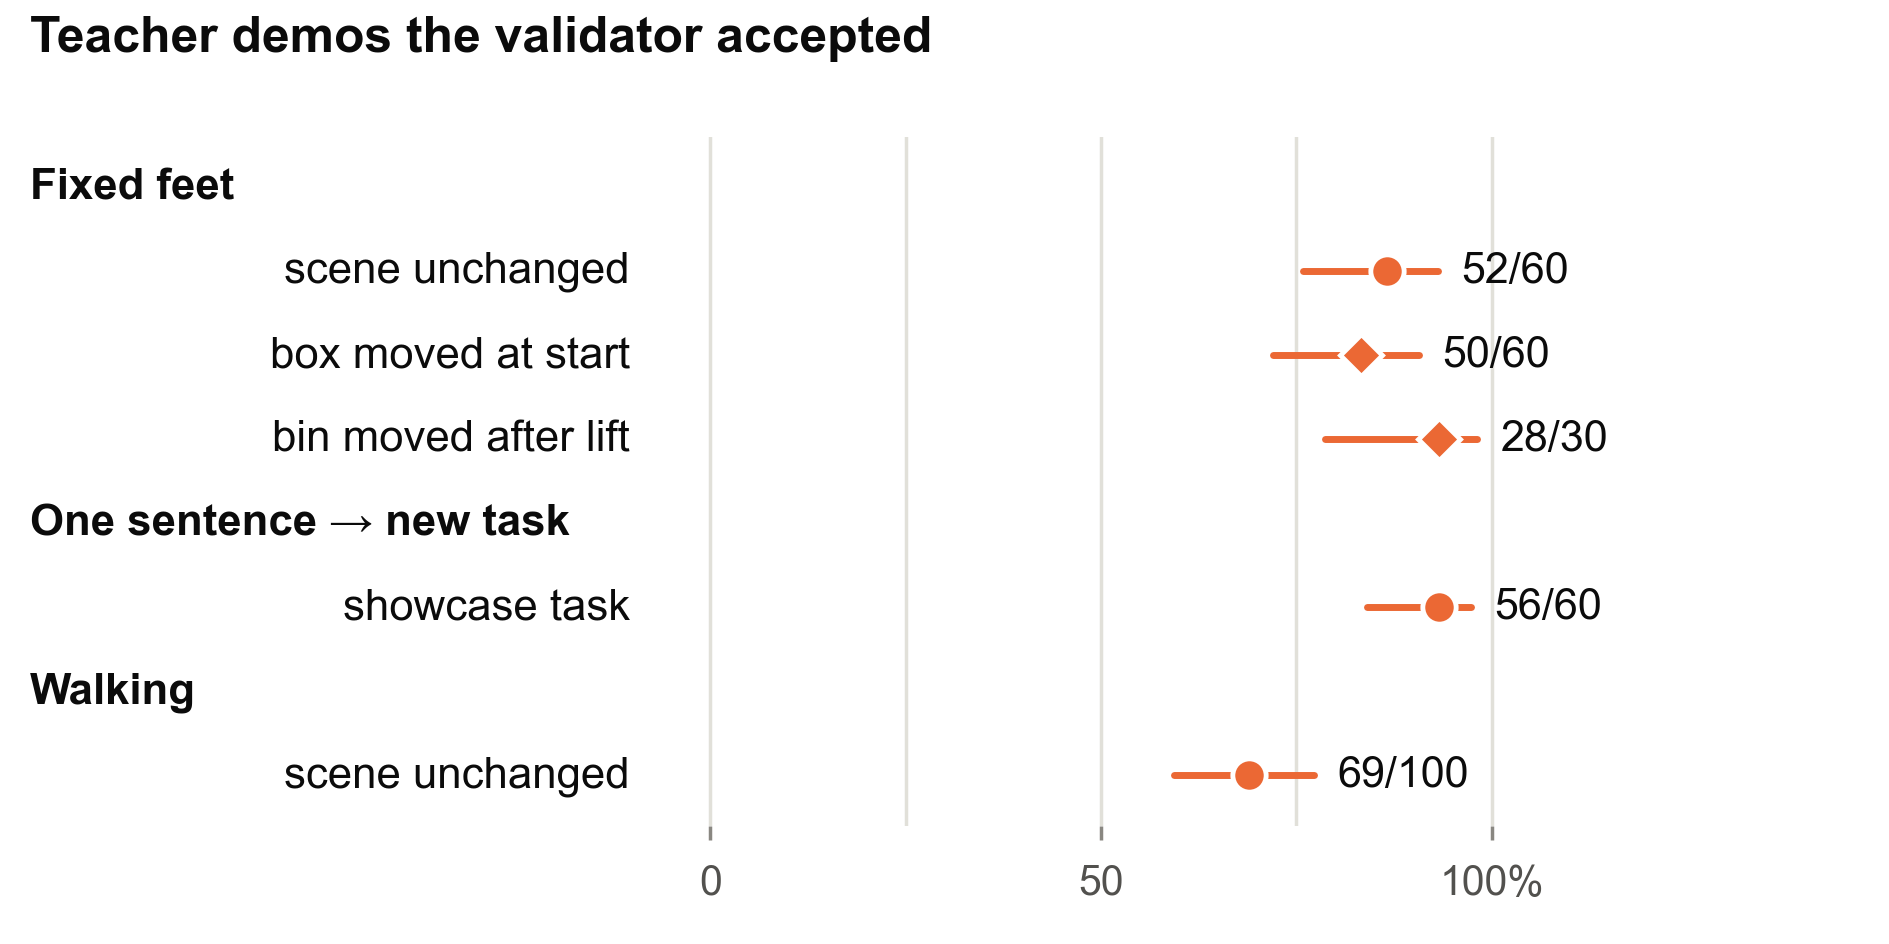
\includegraphics[width=148mm]{teacher-acceptance.png}};
\node[anchor=north west, inner sep=0, text width=148mm] at \at{156}{132} {\T{16}\textbf{The teacher scales:} the validator accepts 56/60 demos for a new task, and 69/100 while walking.};
\foot{Adding recovery and box-moved demos (52 $\rightarrow$ 117) to the fixed-feet student; same seeds, student alone.}
\end{slide}

% 9 ---------------------------------------------------------------------------------------------------------------
\begin{slide}
\slidetitle[Impact]{No humans in the loop. Nothing in the cloud at run time.}
\node[anchor=north, inner sep=0] at \at{160}{42} {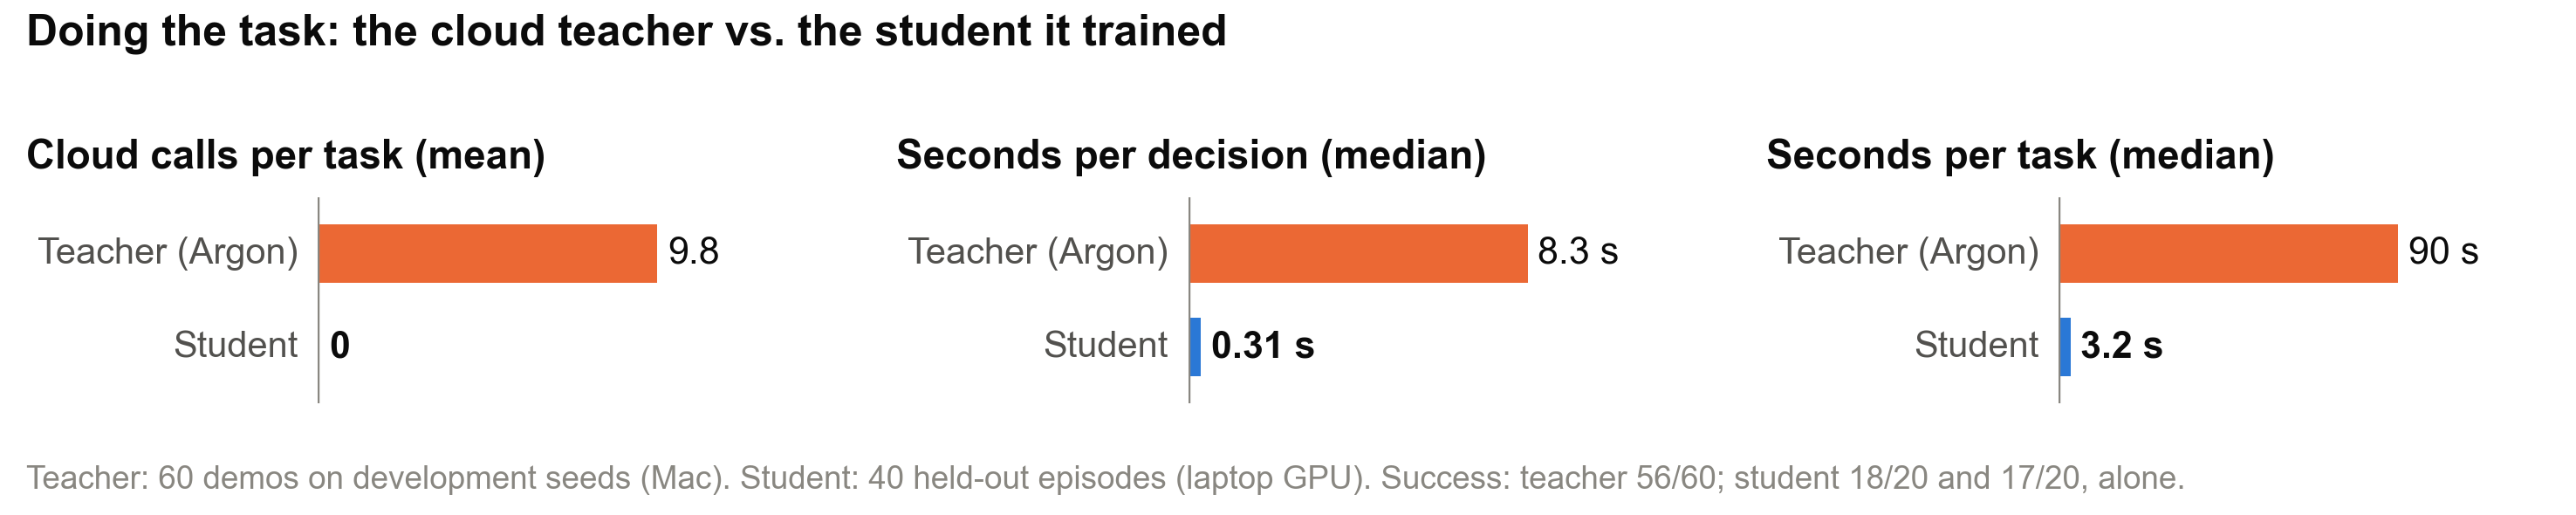
\includegraphics[width=270mm]{impact.png}};
\card{16}{100}{90}{52}{\stat{30}{blue}{1 sentence}\par\vspace{2mm}\T{15}human input: 0 teleoperated steps, 0 labels\par\vspace{1mm}\color{muted}DROID: 50 collectors $\times$ 12 months}
\card{115}{100}{90}{52}{\stat{30}{blue}{20.9 GPU-min}\par\vspace{2mm}\T{15}training, on one laptop GPU\par\vspace{1mm}\color{muted}589 Argon calls for the whole skill}
\card{214}{100}{90}{52}{\stat{30}{blue}{0.31\,s}\par\vspace{2mm}\T{15}per decision, 0 cloud calls\par\vspace{1mm}\color{muted}teacher: 8.3\,s and 9.8 calls per task}
\foot{Teacher: 60 demos on development seeds. Student: 40 held-out episodes. Measured from event logs.}
\end{slide}

% 10 --------------------------------------------------------------------------------------------------------------
\begin{slide}
\slidetitle[Architecture]{Camera in, skills out. Ground truth only for the judge.}
\node[anchor=north, inner sep=0] at \at{160}{44} {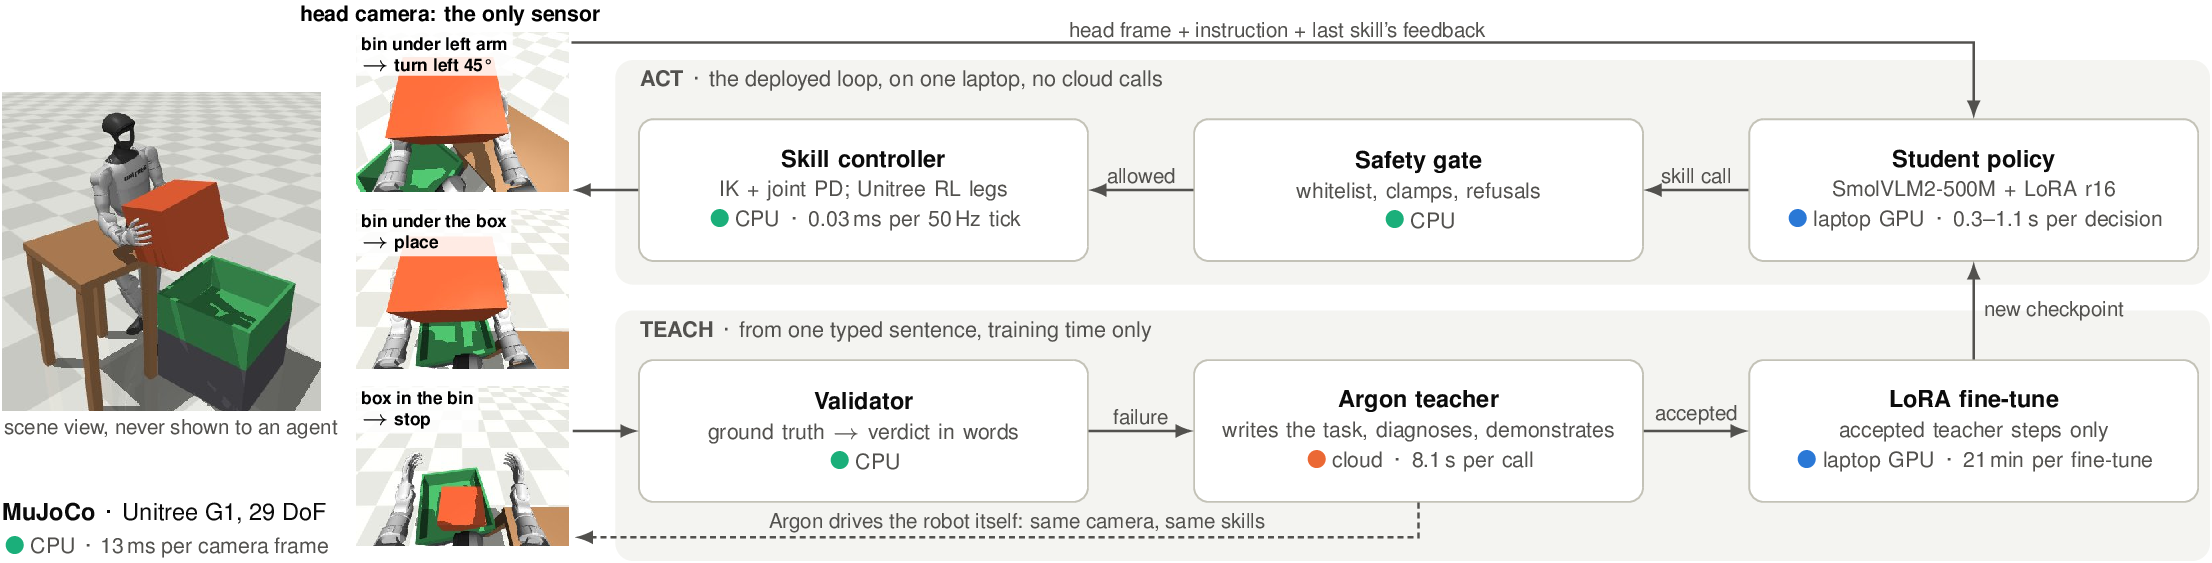
\includegraphics[width=288mm]{architecture.png}};
\card{16}{122}{140}{36}{\T{16}\textbf{Student on the laptop GPU:} 0.31\,s per decision, \textbf{2.01\,GiB of a 3\,GB budget}.}
\card{164}{122}{140}{36}{\T{16}\textbf{Argon in the cloud, teaching only:} 8.1\,s per call. The deployed loop never calls it.}
\end{slide}

% 11 --------------------------------------------------------------------------------------------------------------
\begin{slide}
\slidetitle[Safety and limits]{Safe by construction. Honest about what's next.}
\card{16}{48}{140}{106}{\stat{15}{green}{SAFETY}\par\vspace{4mm}\T{16}\textbf{No stale plans:} every skill is chosen from the newest camera frame.\par\vspace{3mm}\textbf{Refused before anything moves:} past a joint limit, an unreachable target, a walk into the table.\par\vspace{3mm}\textbf{Unsafe demos never train:} the validator rejects falls, limit violations, penetration.\par\vspace{3mm}\textbf{Sealed test seeds}, an 800-call cap, keys never logged; \textbf{600+ tests}.}
\card{164}{48}{140}{106}{\stat{15}{orange}{NEXT}\par\vspace{4mm}\T{16}\textbf{Sim-to-real.} Everything so far is in simulation.\par\vspace{3mm}\textbf{Re-aiming the student.} It keeps its learned routine when the bin moves beyond its training range; the teacher already re-aims.\par\vspace{3mm}\textbf{Walking.} The teacher walks (69/100 demos accepted); the student has its first successes (2/20).}
\end{slide}

% 12 --------------------------------------------------------------------------------------------------------------
\begin{slide}
\node[anchor=center, inner sep=0, text width=290mm, align=center] at ($(current page.center)+(0,34mm)$) {\T{18}\bfseries\color{blue}Scaffld\par};
\node[anchor=center, inner sep=0, text width=290mm, align=center] at ($(current page.center)+(0,4mm)$) {\T{44}\bfseries Teach a robot a new skill\\in 39.7 minutes.\par};
\node[anchor=center, inner sep=0, text width=290mm, align=center] at ($(current page.center)+(0,-28mm)$) {\T{20}\color{muted}One sentence. No human demonstrations. A student that runs alone.\par};
\node[anchor=center, inner sep=0, text width=290mm, align=center] at ($(current page.center)+(0,-50mm)$) {\T{16}github.com/owenbonc/isaac-s-mom\par};
\end{slide}

\end{document}
